\documentclass[journal, a4paper]{IEEEtran}
\usepackage{graphicx}
\usepackage{url} 
\usepackage{amsmath}
\usepackage{subcaption}
\begin{document}

% Define document title and author
	\title{Homework 3: Statistical Parsing with "Unsupervised" Domain Adaptation}
	\author{Guangyu Lin, EID: gl8429
}
	\markboth{CS 388 Natural Language Processing - University of Texas at Austin}{}
	\maketitle

% Write abstract here
\begin{abstract}
	The short report is intended to present homework 3, statistical parsing with "Unsupervised" domain adaptation. When learning statistical parsers, the learned parser can be quite specific to the genre of the training corpus. The author uses a form of semi-supervised learning to solve the task of domain adaption, which is to adapt a system trained on one "source" domain to perform better on a new "target" domain. F1 in this result is compared with different size of seed and self-training set. Our model is trained and tested on the dataset of Wall Street Journal and Brown. Moreover, the author inverts the "source" and "target" corpus and find our model performs much better with larger self-training set.
	
\end{abstract}

% Each section begins with a \section{title} command
\section{Introduction}
\subsection{Self training}

As there is sufficient labeled training data in the source, but there is little or no labeled data for the target, since gathering sufficient training data in every new domain is expensive and labor intensive. We present a form of semi-supervised learning in which a system trained on a "seed" set of labeled data is used to produce automatically labeled output for an unlabelled set of "self-training" data, and the resulting "pseudo-supervised" data is added to the seed training data, and the system is retrained. ~\cite{WEB} Then, we use the retrained model to test our test data. For the toolkit, we use Stanford parser and for the dataset, we use Brown and Wall Journal Street.

The report is organized as following, the experiments are stated in Section~\ref{compare}. The results table and figure is provided in Section~\ref{result}. We discuss our results in Section~\ref{discuss}. And Section~\ref{conclude} is the conclusion of the report.

% Main Part
\section{Implementation}\label{compare}
Our experiments include eight separate experiments. The following title format defines as {\bf \{SeedSet\}\_\{SelfTrainingSet\}\_\{TestSet\}}. And {\bf WSJ} defines as Wall Street Journal, {\bf Brown} defines as Brown and {\bf NO} is an empty set.

For the implementation, we check whether it is trainable for each sentence in the corpus at first, then prepare seed set, self training set, test set as below. The most important part is the {\bf learn} function. We used the seed set to train a {\bf paser} by {\bf LexicalizedParser}, then we labeled the self-training set by this {\bf parser}, finally, we combine the self-training set(labeled) with seed set(correct) to retrain a new {\bf parser}. We use the test set to test the retrain {\bf parser} and calculate the F1.

\subsection{In Domain: WSJ\_NO\_WSJ}
Use WSJ sections 02-22 as labelled seed data and WSJ sections 23 as the test sets.

\subsection{Across Domain: WSJ\_NO\_Brown}
Use WSJ sections 02-22 as labelled seed data and last 10\% of the sentences in each genre of Brown Corpus as the test sets.

\subsection{Unsupervised Domain Adaptation: WSJ\_Brown\_Brown}
Use WSJ sections 02-22 as labelled seed data, the first 90\% of the sentences in each genre as the unlabelled self-training set and the rest 10\% of the sentences as the test sets.

\subsection{Self Training Brown}
Use the first 10000 labeled sentences from WSJ sections 02-22 as seed set, the rest 10\% of the sentences of Brown as the test sets. Additionally, we change the self-training sentences from first 90\% in Brown.

\subsection{In Domain: Brown\_NO\_Brown}
Use the previous 90\% Brown data as the seed set and the rest 10\% Brown data as the test set.

\subsection{Across Domain: Brown\_NO\_WSJ}
Use the previous 90\% Brown data as the seed set and WSJ section 23 as the test set.

\subsection{Unsupervised Domain Adaptation: Brown\_WSJ\_WSJ}
Use the previous 90\% Brown data as the seed set, WSJ sections 02-22 as the self-training data and WSJ section 23 as the test set.

\subsection{Self Training WSJ}
Use the first 10000 labeled sentences from Brown as seed set, the rest 10\% of the sentences of Brown as the test sets. Additionally, we change the self-training sentences from WSJ sections 02-22.

\section{Experiment Results}\label{result}

We present the eight experiments' results in \ref{compare}. Additionally, we also present how many words we added for self-training, how many words we retrain and the running time of different seed set.

	\begin{table}[!hbt]
		\begin{center}
		% Title of the table
		\caption{WSJ\_NO\_WSJ}
		\label{tab:1}
		\begin{tabular}{|c|c|c|c|c|}
			\hline
			Seed Size & Added & Total & $F_{1}$ & time\\ \hline
			  1000  & 0.0 & 26002 & 0.717 & 282\\ \hline
			  2000  & 0.0 & 51235 & 0.766 & 355\\ \hline
			  3000  & 0.0 & 76152 & 0.779 & 423\\ \hline
			  4000  & 0.0 & 101881 & 0.790 & 535\\ \hline
			  5000  & 0.0 & 127107 & 0.797 & 606\\ \hline
			  7000  & 0.0 & 179946 & 0.806 & 727\\ \hline
			  10000  & 0.0 & 256268 & 0.811 & 1010\\ \hline
			  13000  & 0.0 & 333723 & 0.820 & 1143\\ \hline
			  16000  & 0.0 & 408679 & 0.824 & 1328\\ \hline
			  20000  & 0.0 & 509117 & 0.829 & 1507\\ \hline
			  25000  & 0.0 & 635765 & 0.831 & 1796\\ \hline
			  30000  & 0.0 & 761256 & 0.835 & 1681\\ \hline
			  35000  & 0.0 & 888088 & 0.835 & 1936\\
			 \hline
		\end{tabular}
		\end{center}
		\vspace{-5mm}
	\end{table}

	\begin{table}[!hbt]
		\begin{center}
		% Title of the table
		\caption{WSJ\_NO\_Brown}
		\label{tab:2}
		\begin{tabular}{|c|c|c|c|c|}
			\hline
			Seed Size & Added & Total & $F_{1}$ & time\\ \hline
			  1000  & 0.0 & 26002 & 0.670 & 2343\\ \hline
			  2000  & 0.0 & 51235 & 0.700 & 434\\ \hline
			  3000  & 0.0 & 76152 & 0.711 & 624\\ \hline
			  4000  & 0.0 & 101881 & 0.726 & 706\\ \hline
			  5000  & 0.0 & 127107 & 0.728 & 776\\ \hline
			  7000  & 0.0 & 179946 & 0.738 & 876\\ \hline
			  10000  & 0.0 & 256268 & 0.756 & 1229\\ \hline
			  13000  & 0.0 & 333723 & 0.762 & 1277\\ \hline
			  16000  & 0.0 & 408679 & 0.769 & 1462\\ \hline
			  20000  & 0.0 & 509117 & 0.771 & 1702\\ \hline
			  25000  & 0.0 & 635765 & 0.776 & 1981\\ \hline
			  30000  & 0.0 & 761256 & 0.778 & 2252\\ \hline
			  35000  & 0.0 & 888088 & 0.783 & 2542\\
			 \hline
		\end{tabular}
		\end{center}
		\vspace{-5mm}
	\end{table}
	
		\begin{table}[!hbt]
		\begin{center}
		% Title of the table F
		\caption{WSJ\_Brown\_Brown}
		\label{tab:3}
		\begin{tabular}{|c|c|c|c|c|}
			\hline
			Seed Size & Added & Total & $F_{1}$ & time\\ \hline
			  1000  & 409674 & 435676 & 0.686 & 4143\\ \hline
			  2000  & 409674 & 460909 & 0.713 & 4434\\ \hline
			  3000  & 409674 & 485826 & 0.724 & 4624\\ \hline
			  4000  & 409674 & 511555 & 0.730 & 5706\\ \hline
			  5000  & 409674 & 536781 & 0.743 & 6776\\ \hline
			  7000  & 409674 & 589620 & 0.748 & 7876\\ \hline
			  10000  & 409674 & 665942 & 0.760 & 8229\\ \hline
			  13000  & 409674 & 743397 & 0.772 & 9277\\ \hline
			  16000  & 409674 & 818353 & 0.780 & 10462\\ \hline
			  20000  & 409674 & 918791 & 0.783 & 10702\\ \hline
			  25000  & 409674 & 1045439 & 0.785 &11981\\ \hline
			  30000  & 409674 & 1170932 & 0.785 & 11252\\ \hline
			  35000  & 409674 & 1297696 & 0.790 & 12542\\
			 \hline
		\end{tabular}
		\end{center}
		\vspace{-5mm}
	\end{table}
	
	\begin{table}[!hbt]
		\begin{center}
		% Title of the table
		\caption{Self Training Brown}
		\label{tab:4}
		\begin{tabular}{|c|c|c|c|c|}
			\hline
			Seed Size & Added & Total & $F_{1}$ & time\\ \hline
			  1000  & 23490 & 279758 & 0.761 & 7670\\ \hline
			  2000  & 49834 & 329592 & 0.759 & 4406\\ \hline
			  3000  & 75155 & 404747 & 0.760 & 23876\\ \hline
			  4000  & 100075 & 504822 & 0.759 & 2448\\ \hline
			  5000  & 128000 & 632822 & 0.761 & 2742\\ \hline
			  7000  & 170848 & 803670 & 0.762 & 3032\\ \hline
			  10000  & 224292 & 1027962 & 0.764 & 3591\\ \hline
			  13000  & 275149 & 1303111 & 0.761 & 4075\\ \hline
			  17000  & 342499 & 1645610 & 0.762 & 3723\\ \hline
			  21000  & 419897 & 2065507 & 0.763 & 5113\\
			 \hline
		\end{tabular}
		\end{center}
		\vspace{-5mm}
	\end{table}
	
	\begin{table}[!hbt]
		\begin{center}
		% Title of the table
		\caption{Brown\_NO\_Brown}
		\label{tab:5}
		\begin{tabular}{|c|c|c|c|c|}
			\hline
			Seed Size & Added & Total & $F_{1}$ & time\\ \hline
			  1000  & 0.0 & 23490 & 0.699 & 171\\ \hline
			  2000  & 0.0 & 49834 & 0.730 & 335\\ \hline
			  3000  & 0.0 & 75155 & 0.750 & 407\\ \hline
			  4000  & 0.0 & 100075 & 0.766 & 504\\ \hline
			  5000  & 0.0 & 128000 & 0.772 & 650\\ \hline
			  7000  & 0.0 & 170848 & 0.785 & 814\\ \hline
			  10000  & 0.0 & 224292 & 0.796 & 982\\ \hline
			  13000  & 0.0 & 275149 & 0.801 & 1116\\ \hline
			  17000  & 0.0 & 342499 & 0.807 & 1323\\ \hline
			  21000  & 0.0 & 419897 & 0.811 & 1567\\
			 \hline
		\end{tabular}
		\end{center}
		\vspace{-5mm}
	\end{table}
	
	\begin{table}[!hbt]
		\begin{center}
		% Title of the table
		\caption{Brown\_NO\_WSJ}
		\label{tab:6}
		\begin{tabular}{|c|c|c|c|c|}
			\hline
			Seed Size & Added & Total & $F_{1}$ & time\\ \hline
			  1000  & 0.0 & 23490 & 0.644 & 196\\ \hline
			  2000  & 0.0 & 49834 & 0.683 & 392\\ \hline
			  3000  & 0.0 & 75155 & 0.700 & 541\\ \hline
			  4000  & 0.0 & 100075 & 0.710 & 657\\ \hline
			  5000  & 0.0 & 128000 & 0.718 & 810\\ \hline
			  7000  & 0.0 & 170848 & 0.731 & 1092\\ \hline
			  10000  & 0.0 & 224292 & 0.730 & 1303\\ \hline
			  13000  & 0.0 & 275149 & 0.736 & 1422\\ \hline
			  17000  & 0.0 & 342499 & 0.743 & 1775\\ \hline
			  21000  & 0.0 & 419897 & 0.745 & 6088\\
			 \hline
		\end{tabular}
		\end{center}
		\vspace{-5mm}
	\end{table}
	
		\begin{table}[!hbt]
		\begin{center}
		% Title of the table
		\caption{Brown\_WSJ\_WSJ}
		\label{tab:7}
		\begin{tabular}{|c|c|c|c|c|}
			\hline
			Seed Size & Added & Total & $F_{1}$ & time\\ \hline
			  1000  & 898178 & 921668 & 0.663 & 10125\\ \hline
			  2000  & 898178 & 948012 & 0.697 & 8346\\ \hline
			  3000  & 898178 & 973333 & 0.715 & 8537\\ \hline
			  4000  & 898178 & 988253 & 0.730 & 8627\\ \hline
			  5000  & 898178 & 1026178 & 0.739 & 9815\\ \hline
			  7000  & 898178 & 1069026 & 0.742 & 9042\\ \hline
			  10000  & 898178 & 1122470 & 0.740 & 10323\\ \hline
			  13000  & 898178 & 1173327 & 0.746 & 11442\\ \hline
			  17000  & 898178 & 1240677 & 0.753 & 12774\\ \hline
			  21000  & 898178 & 1318075 & 0.758 & 13889\\
			 \hline
		\end{tabular}
		\end{center}
		\vspace{-5mm}
	\end{table}
	
			\begin{table}[!hbt]
		\begin{center}
		% Title of the table
		\caption{Self Training WSJ}
		\label{tab:8}
		\begin{tabular}{|c|c|c|c|c|}
			\hline
			Seed Size & Added & Total & $F_{1}$ & time\\ \hline
			  1000  & 21475 & 245767 & 0.742 & 6184\\ \hline
			  2000  & 47533 & 271825 & 0.747 & 6392\\ \hline
			  3000  & 72163 & 296455 & 0.750 & 6541\\ \hline
			  4000  & 99373 & 324367 & 0.752 & 6657\\ \hline
			  5000  & 111976 & 352292 & 0.749 & 6810\\ \hline
			  7000  & 160925 & 395140 & 0.753 & 8092\\ \hline
			  10000  & 213756 & 448548 & 0.759 & 8303\\ \hline
			  13000  & 268246 & 499441 & 0.762 & 9422\\ \hline
			  17000  & 332565 & 566791 & 0.761 & 9775\\ \hline
			  21000  & 407864 & 644189 & 0.762 & 9988\\
			 \hline
		\end{tabular}
		\end{center}
		\vspace{-5mm}
	\end{table}
	
	
\section{Discussion}\label{discuss}
We draw Figure~\ref{plot1}.a with Table. ~\ref{tab:1}, Table.~\ref{tab:2} and Table.~\ref{tab:3} to compare the results of normal training and testing on WSJ, normal training on WSJ and testing on Brown and unsupervised domain adaptation by normal training on WSJ, self-training on Brown and then testing on Brown. And we also draw Figure~\ref{plot2}.a with Table.~\ref{tab:4}, which is experiment on increasing the size of the self-training set.

When we do the in domain training and testing, F1 score is range from 0.717 to 0.835 and we also found that F1 score increase by the increasing of the seed set size. However, when the seed set is larger, the F1 score won't increase as much as before. When we shift from testing on WSJ to testing on Brown, we found F1 score drop not much, which is range from 4\% - 5\%. And F1 score also positive related to the seed set size with out-of-domain testing, which is range from 0.670 - 0.783. Additionally, we found the running time of in-domain testing is a little shorter than out-of-domain testing, which is because in-domain testing converges earlier. And the running time increase about 7 time between 1000 sentences seed size and 35000 sentences seed size, which causes of the larger the seed set is the longer training time we need. This is a trade-off between F1 score and running time.

We found that self-training always helps improve performance, however not much, which is only 1\% to 2\%, as we increase the seed set, which show the characteristic of EM. Additionally, the running time really increases a lot because, we need to labelled a lot of data and retrain a large dataset. So we think, if we don't care much about that 1\% improvement, adding a small amount of self training data is enough.

We can get more clear result from Figure~\ref{plot2}.a. We found that the range of F1 score is among 0.759 to 0.764 with different self-training set, which reflects the size of self-training set doesn't improve F1 score a lot, but the overall trend is indeed improve.

Therefore, from Figure~\ref{plot1}.a and Figure~\ref{plot2}.a, we find that the size of seed set will improve F1 score a lot, which almost 15\%, however, the increasing size of self-training set may not be very helpful, though it really improve 1\%-2\%.

The we inverted the "source" and "target" and draw Figure\ref{plot1}.b and Figure\ref{plot2}.b by Table.\ref{tab:5} - Table.\ref{tab:8}. The normal trend is almost similar to the previous one. However, we found that the F1 score of  Brown corpus is a little worse than WSJ corpus on average. It may caused be the less training words each time, we can find the total words in WSJ, which we train with same number of sentences of seed set, is a little larger than the total words in Brown. For example, when we have 10000 sentences, we train 256268 words in WSJ, compared with 224292 words in Brown. Therefore, we can conclude that the size of the training words influence F1 score a lot.

Compared with Reichart and Rappoport's paper~\cite{EXPERT}, we found that there is not much difference where the self-training set from Brown of WSJ. And my result is better than Reichart's because my seed set is much larger. Overall, Reichart's paper also shows the average F1 score of WSJ is better than the average F1 score of Brown with the same sentences size of training and test.
Additionally, self-training improves F1 score more than me in Reichart and Rappoport's paper. I think the reason may be the small seed set they trained.

\begin{figure}
        \begin{subfigure}[b]{0.24\textwidth}
                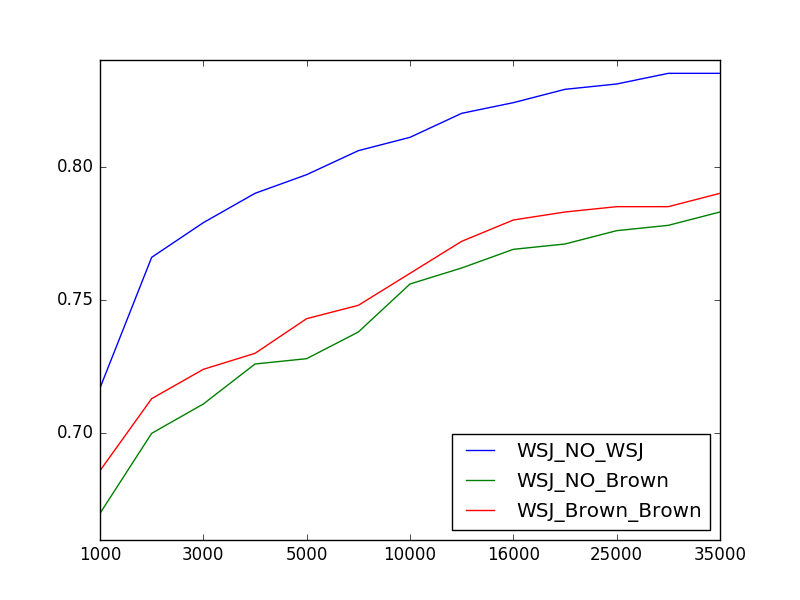
\includegraphics[width=\linewidth]{plot1}
                \caption{Comparison with normal training and testing on WSJ, normal training on WSJ and testing on Brown and unsupervised domain adaptation by normal training on WSJ, self-training on Brown and then testing on Brown}
                \label{fig:gull}
        \end{subfigure}%
        \hspace{\fill}
        \begin{subfigure}[b]{0.24\textwidth}
                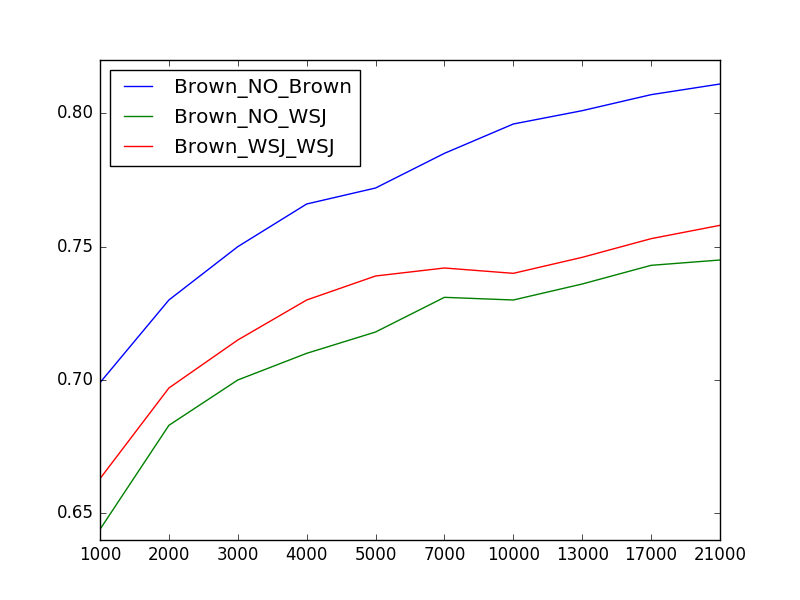
\includegraphics[width=\linewidth]{plot3}
                \caption{Comparison with normal training and testing on Brown, normal training on Brown and testing on WSJ and unsupervised domain adaptation by normal training on Brown, self-training on Brown and then testing on WSJ}
                \label{fig:tiger}
        \end{subfigure}%
        \caption{}\label{plot1}
\vspace{-2mm}
\end{figure}


\begin{figure}
        \begin{subfigure}[b]{0.24\textwidth}
                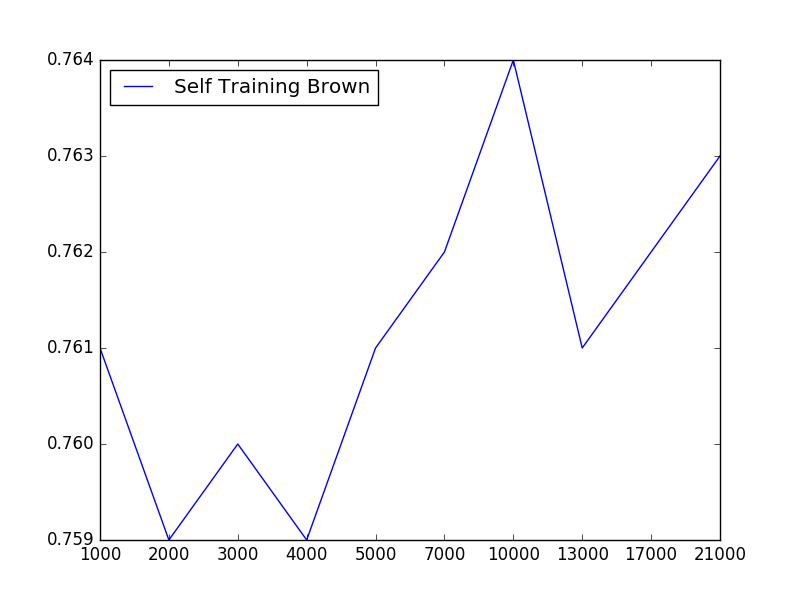
\includegraphics[width=\linewidth]{selfBrown}
                \caption{Increasing the size of the self-training set in Brown}
                \label{fig:gull2}
        \end{subfigure}%
        \hspace{\fill}
        \begin{subfigure}[b]{0.24\textwidth}
                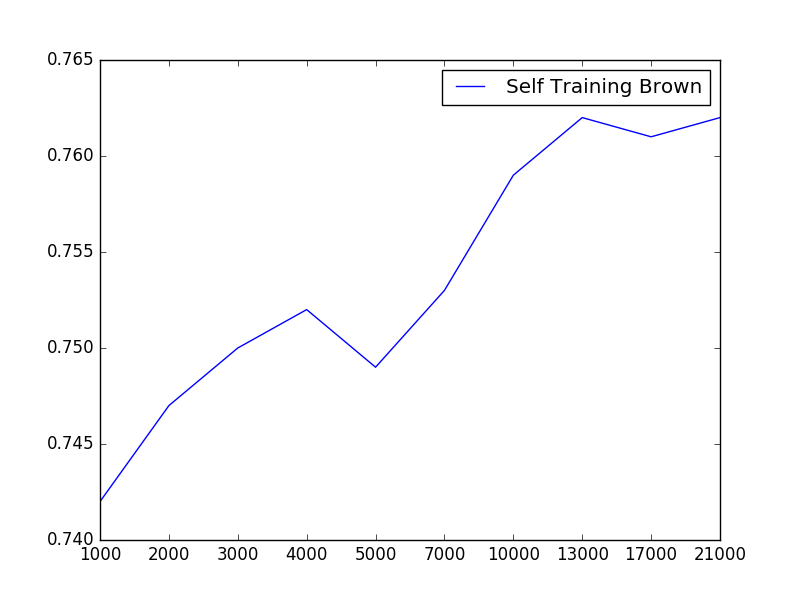
\includegraphics[width=\linewidth]{selfWSJ}
                \caption{Increasing the size of the self-training set in WSJ}
                \label{fig:mouse}
        \end{subfigure}
        \caption{}\label{plot2}
\vspace{-2mm}
\end{figure}

\section{Conclusion}\label{conclude}
	In this report, we talked about eight different experiments with normal in-domain training and testing, normal out-domain training and testing, and unsupervised domain adaptation by out-domain training, self-training and testing. Additionally, we also experiments on different size of self-training and compared the results. To make a common conclusion, we also invert the "source" and "target" between Wall Street Journal and Brown corpus. And compared our results with Reichart and Rapporport's paper. In the end, we find larger seed set will improve F1 score a lot. Self training will also be helpful to out-domain experiment, but not very much. There is also a trade off between F1 score and the running time. We should give a propriate seed size and self-training size within our purpose.
% Now we need a bibliography:
\begin{thebibliography}{5}

	%Each item starts with a \bibitem{reference} command and the details thereafter.
	\bibitem{WEB} % Transaction paper
	https://www.cs.utexas.edu/~mooney/cs388/hw3.html
	
	\bibitem{EXPERT}
	Reichart, Roi, and Ari Rappoport. "Self-training for enhancement and domain adaptation of statistical parsers trained on small datasets." ACL. Vol. 7. 2007.

\end{thebibliography}


% Your document ends here!
\end{document}